 %%% machine_learning_p3.tex
%%%
%%% This LaTeX source document can be used as the basis for your technical
%%% paper or abstract. Intentionally stripped of annotation, the parameters
%%% and commands should be adjusted for your particular paper - title, 
%%% author, article DOI, etc.
%%% The accompanying ``template.annotated.tex'' provides copious annotation
%%% for the commands and parameters found in the source document. (The code
%%% is identical in ``template.tex'' and ``template.annotated.tex.'')

\documentclass[annual]{acmsiggraph}

\TOGonlineid{45678}
\TOGvolume{0}
\TOGnumber{0}
\TOGarticleDOI{1111111.2222222}
\TOGprojectURL{}
\TOGvideoURL{}
\TOGdataURL{}
\TOGcodeURL{}

\title{Unsupervised Learning and Dimensionality Reduction Analysis}

\author{Daniel A. Castro (dcastro9@gatech.edu) \\ CS-4641 - Machine Learning}
\pdfauthor{Daniel A. Castro}

\keywords{machine learning, cs4641, unsupervised learning, dimensionality reduction}

\begin{document}

\maketitle

\begin{abstract}
Unsupervised Learning and Dimensionality Reduction are sections of Machine Learning that focuses on learning from and improving the data.  Overall, the methods in this analysis focus on clustering data without prior knowledge of its classification. The datasets in this analysis will be strictly medical, and more specifically, focus on breast cancer diagnosis. The two datasets approach the classification problem of breast masses differently, which will hopefully better expose the importance of how you categorize your problem. For clustering, I will use k-means clustering and expectation maximization (EM) in order to diagnose the datasets into clusters. For dimensionality reduction, I will use principal component analysis (PCA), independent component analysis (ICA), Random Projections (RP), and Random Subsets (RS). I will complete my analyis with an evaluation of these methods by comparing the results of one of the datasets on a Multilayer Perceptron classification (a type of neural network), and explain the advantages and disadvantages that the clustering and dimensionality reduction algorithms may have on these data sets.
\end{abstract}

\section{Introduction}
In my previous work, \cite{Castro1:2013} and \cite{Castro2:2013}, I focused on applying algorithms to the data in an attempt to generate a function which was capable of classifying the data. In this case however, our data does not have classifications. I also begin to introduce the concept of dimensionality reduction with a very brute method of random subsets, which is improved upon in this analysis by actually randomly selecting attributes in order to see the effect it has on the performance of the dataset.
\section{Background Information}
In this analysis I do cover a number of different algorithms which are relatively simple to explain conceptually. I will do a basic explanation of each of the algorithms involved, and further mention how the algorithms were implemented and what publicly available software was used in order to implement them. The only algorithm which will not be covered will be the multilayer perceptron, which is the neural network we use as our evaluation metric, available on Weka. For a better explanation of the algorithm, see \cite{Castro1:2013}.
\subsection{Clustering Algorithms}
For the clustering algorithms, I used the implementations in the publicly available Weka library, ~\cite{Hall_weka:2010}.
\subsubsection{K-Means Clustering}
K-Means clustering is a very simple, yet powerful algorithm for clustering a number of attributes into k clusters. A simple way of implementing the algorithm is to choose k points from your data, and assign those to be the centroid of each cluster. Then, classify each point to one of the clusters, based on a distance metric (generally the Euclidean distance). Once this is done, you recalculate the center (average) of each of the clusters, and assign that to be the centroid. You reclassify all of your points, and continue to iterate this procedure until it converges. In this case, you are required to know the number of clusters you want to classify these into, and so for both of our datasets, I set this to 2, given that our data was a binary classification problem. Further, I used two distance metrics, the Manhattan distance, and the Euclidean distance, but neither of them had a significant performance gain over the other for all of the experiments.
\subsubsection{Expectation Maximization (EM)}
Expectation Maximization (EM) focuses on the probability that the data that I could have seen a certain phenomenon, assuming that I have not seen it. EM actually tries to apply a certain model or distribution to your data in order to represent the information. In this experiment, I allowed EM to assign however many clusters it determined was adequate to the data, but these results were difficult to evaluate. Given this difficulty, I also ran EM with the assumption that our data could be divided into two clusters (the two distributions, benign and malignant), and used that to analyze the performance of the algorithm. It is important that although this method of evaluation makes it easily comparable to other methods, it hides some of the advantages of EM which will be covered in the analysis.
\subsection{Dimensionality Reduction Algorithms}
Dimensionality Reduction algorithms focus on restructuring the input data prior to classifying it with learning algorithms.
\subsubsection{Principal Component Analysis (PCA)}
Principal Component Analysis creates a new coordinate system which maximizes the distance between the clusters of information, based on the components of the data (attributes). I used the implementation available in the Weka library.
\subsubsection{Independent Component Analysis (ICA)}
Independent Component Analysis focuses on restructuring the input data by increasing the separation between each of the components from one another. The metric I use for separation changes the dynamic of the algorithm, but the theory behind it is still, for the most part, the same. Our implementation of ICA was available in the ABAGAIL Java Library, and only required minor modifications (the implementation of ARFF output) to run for my application.
\subsubsection{Random Projections (RP)}
Random Projection, put simply, projects a dataset with \emph{n} attributes to a k-dimensional space, where k is inherently lower than \emph{n}. This method works surprisingly well for some approaches, and given that its projection of the data to lower dimensions, it is nearly guaranteed to improve the computation time of the algorithm (although this doesn't say much for its accuracy). Depending on the projection, the algorithm may not be heavily affected in its accuracy, but reasonably, accuracy will tend to decrease as \emph{n} approaches 1. I used the implementation available in Weka, which allowed for the saving of the processed data files, which I use later in the assignment for the analysis of neural networks after dimensionality reduction.
\subsubsection{Random Subsets (RS)}
Lastly, I chose random subsets because of the analysis that had previously been done in previous work~\cite{Castro1:2013}. This algorithm simply chooses a subset of the attributes (which is taken as input). The instant guarantee is faster computation, but its performance will generally suffer because of it.
\subsection{Datasets}
For this analysis, I chose one of the datasets from~\cite{Castro1:2013}. This dataset focused on categorizing breast masses as malignant or benign. That stated, I chose a second breast mass classification dataset based on mammographies introduced in~\cite{elter2007prediction}. The two datasets approach the categorization of breast masses differently, which I did purposefully in order to better understand what parameters are best for the classification of breast masses.
\subsubsection{Wisconsin Breast Cancer (Diagnostic Dataset)}
This dataset is composed of 30 attributes, and 569 instances, of which 357 are benign classifications, and 212 are malignant classifications. The attributes are actually best described by 10 parameters that identify the cell nucleus, and for each of these parameters the data provides its standard deviation and its worst error. For more information about this dataset, see ~\cite{Castro1:2013}. Due to the similarity of these two datasets, from hereon, this dataset will be referred to as the \emph{Wisconsin Dataset}.
\subsubsection{Mammographic Mass Dataset}
The mammographic mass dataset is composed of 5 attributes (the 6th one is the classificaiton variable), and a total of 961 instances of which 516 are benign and 445 are malignant. The attributes are determined from the Breast Imaging Reporting and Data System (BI-RADS) which is a system developed to ensure the quality of mammographies. In addition to that assessment (which is on a ordinal scale of 1-6) they focus on the shape of the mass, but also include the age of the patient. It is important to note that the dataset is partially incomplete. Given that some algorithms were unable to process incomplete data, these values were replaced with -1 (since all of the parameters were on a positive integer scale). I do acknowledge that this may have a negative effect on some classifications by clustering data points with missing data from the data points that are complete, but also note that uniquely identifying missing data points could also have a benefit given that the number of complete attributes outnumber those that are missing certain attributes. From hereon, this dataset will be referred to as the \emph{Mammography Dataset}.
\section{Clustering Algorithms}
The first experiments I conducted were with clustering. In order to properly evaluate these experiments, I set the clustering of the algorithms to two clusters, and then compared to the classification attribute. It goes without saying that the classification attribute was removed prior to doing every experiment (otherwise clustering would be trivial). A significant portion of the performance of clustering was due to the problems I chose which lend themselves to strictly two clusters (relatively simple). However, the Mammography dataset makes this problem a little bit more difficult due to missing data, which highlights the overall performance dip in comparison to the Wisconsin dataset. 
\subsection{K-Means Clustering}
For k-means clustering, I felt like the dimensionality of the problem would be the biggest factor in defining a better classification. For that matter, the Wisconsin Dataset would, in my hypothesis, have a higher level of accuracy, given that it has 30 attributes, in comparison to the Mammography Dataset which only contains 5 attributes.
\begin{figure}[ht]
  \centering
  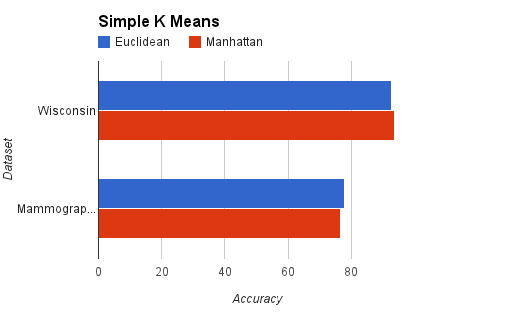
\includegraphics[width=3.5in]{charts/k-means-comparison.png}
  \caption{This illustrates that the Manhattan and Euclidean distances had negligible effects, but in both instances the Wisconsin Dataset outperformed the Mammography dataset, which can be explained due to the disparity in the number of attributes between the datasets.}
  \label{fig:clust1}
\end{figure}
The hypothesis is verified in Figure~\ref{fig:clust1}, which demonstrate the higher performance of the Wisconsin dataset. It is further important to note that the Mammography dataset has nearly twice the number of data points, which indicates that a lack of data could not have caused the differing performance. However, it may be the case that the missing attributes distributed throughout the Mammography dataset do have a negative effect in its overall classification which was not only seen here but throughout all of the experiments conducted.
\subsection{Expectation Maximization (EM)}
In expectation maximization, I expected to see an overall better performance than with k-means clustering. I believe it won't be as evident in the Wisconsin Dataset because of its already significantly low error, but more so in the Mammography dataset. EM was run without a cluster specified, and returned very poor results for the Wisconsin Dataset (at 25\% correct), and decently better for the Mammography dataset (67\% correct). These accuracy results are inherently flawed because the classification can only be mapped to two clusters, which means that because the Wisconsin Dataset gets classified to 13 datasets, only two of them can be attributed for classification, and hence the error. The Mammography dataset, in contrast, gets mapped to 5 clusters, and the two that are attributed take up 81\% of the attributes, which therefore explains the accuracy.
\begin{figure}[ht]
  \centering
  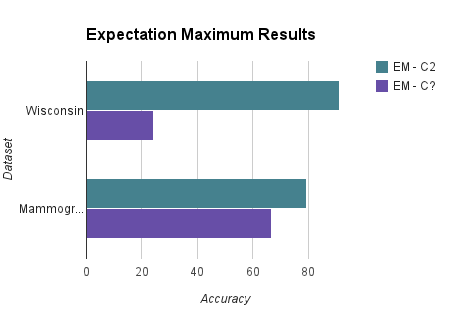
\includegraphics[width=3.5in]{charts/em_result.png}
  \caption{This demonstrates that the performance of EM without a target number of clusters tends to return erroneous results. The results for both of the datasets, assuming I supply a cluster size of 2, are not experimentally significant in comparison to simple k-means. In this figure's key, C? represents the act of not specifying a cluster size and letting the algorithm determine it.}
  \label{fig:clust2}
\end{figure}

In this case, the complexity of the Wisconsin Dataset hurts its performance given that it is too difficult to map a model to each attribute with a somewhat limited number of instances. I believe its accuracy would improve had the dataset been originally larger. This theory is confirmed by the performance of the Mammography dataset, which is both less complex, and has more attributes. Further, for comparison, I assign the cluster size to be 2, and compare the results to the correct classes. The results do not prove to be as significant as my original hypothesis predicted.
As can be seen in Figure~\ref{fig:clust2}, the results due to EM do not significantly improve the results. This may be due to the general lack of data and excessive attributes. For the Mammography dataset, the missing parameters in some of the instances weaken its peformance despite it being a slightly bigger dataset. In contrast, for the Wisconsin Dataset, the number of attributes is significantly bigger (6 times) and the number of instances is halved. The dimensionality reduction algorithms may help the performance of the Wisconsin Dataset, and that is what I will cover next.
\section{Dimensionality Reduction Algorithms}
The Dimensionality Reduction algorithms focus on changing the structure of the input data prior to processing it with a learning algorithm, which in our case, will be processed with a multilayer perceptron (neural network).
\subsection{PCA}
PCA actually reduces the Wisconsin dataset from 30 attributes to 10 attributes or comparatively by 66\%. PCA produces a very interesting result in the data, wherein the distribution of its attributes focus heavily on the standard error. This is intriguing because of how the Wisconsin dataset is setup. One would think the mean of the value would be the most important value but a significant portion of the attributes for PCA rely on the standard error, which explains the distribution of the data in a different light.

In contrast, it does not reduce the number of attributes of the Mammography dataset, which will provide an interesting change for the clustering algorithms. 
\subsection{ICA}
ICA took as an input the number of attributes that the dataset should be reduced to. For the purpose of analysis, I reduced the Wisconsin Dataset to five different number of attributes, 1, 3, 5, 10, and 15. The same was done for the Mammography Dataset, except that I reduced it to 1, 2, 3, and 4 (given that the maximum I could reduce it was 4).
\subsection{Random Projections}
For Random Projections, a very similar approach was taken (in comparison to ICA). I randomly projected to 5, 10, 15, 20, and 25 attributes for the Wisconsin Dataset, and randomly projected the Mammography dataset to 1, 2, 3, and 4. Due to its randomness, I ran random projections numerous times on 25 attributes, and observed an interesting phenomenon where the data would project to what seemed to be a mirror image of itself but on the left or right of the distribution. I also noticed that the data seemed to map a normal distribution shifted left or right, which may explain why, for the Wisconsin dataset, on two clusters, it was 91.2\% accurate (results can be seen in Figure~\ref{fig:clust2}).
\subsection{Random Subsets}
Lastly, for Random Subsets, I focused on only choosing a constant number of attributes, but three iterations (since its random, it provides three unique results). For the Wisconsin Dataset I chose to focus on 10 attributes (given the construction of the dataset this made reasonable sense), and for the Mammography Dataset I chose 3 attributes because any less would have made the dataset too difficult, and any more would have made the random subset be too similar to the original dataset.
\section{Clustering with Dimensionality Reduction}
In this section I cover the clustering experiments I ran after conducting dimensionality reduction. We will analyze a variety of the parameters that we altered for some of the reduction algorithms, in order to see the effect that the different number of attributes may have on accuracy and performance. Reproducing these results after dimensionality reduction produced different levels of accuracy, from which we inferred they produced different clusters. However, the performance difference wasn't significant enough for me to interpret that the clusters were vastly different. What I believe is happening in this scenario is that the clusters are more tightly knit together due to the reduction of dimensions, which therefore explains why some data points may change their clusters, and therefore render a change in the results. ICA and PCA are the most heavily affected by the change in dimensionality reduction, and we attribute this to the loss of components that may have been significant to the accuracy of these algorithms prior to reducing dimensions.
\subsection{K-Means Clustering}
For K-Means Clustering, I expected the lower number of attributes due to the random algorithms for the Wisconsin Dataset to decrease its performance more so than the potential change in performance that ICA and PCA may cause. Due to the sheer magnitude of our results, Figure~\ref{fig:kmeanscluster} shows the best results for ICA, RP, and RS out of all of the parameters (number of attributes, for both Euclidean and Manhattan space). For PCA, we simply pick the best out of the Euclidean vs. Manhattan space, which for our results was not a significant difference.

\begin{figure}[ht]
  \centering
  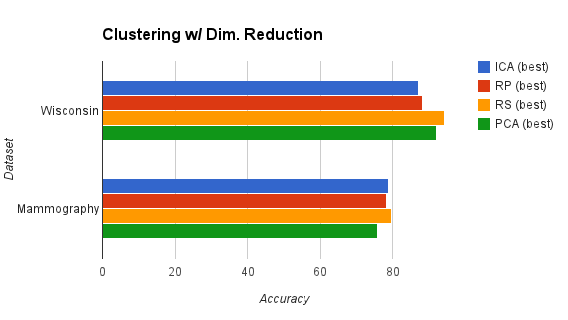
\includegraphics[width=3.5in]{charts/clust_dim_red.png}
  \caption{This demonstrates the accuracy after performing clustering and dimensionality reduction. for k means. The best result out of the Manhattan and Euclidean distance were picked.}
  \label{fig:kmeanscluster}
\end{figure}

The best results bring to light a lot of interesting results that I personally did not expect. It allows us to further analyze our data and better understand how it is composed. First off, the range of accuracy (precision) of the Wisconsin dataset demonstrates a worthwhile characteristic about its composition. More specifically, in ICA, the distance measurement was actually incredibly significant in the classification of the data. This is of particular interest because the main difference between the Manhattan distance measure and the Euclidean distance measure is the alternate paths between certain points. For the Manhattan Distance, the shortest path is the only one that is considered, which may devalue the significance of certain attributes. For random projections, the larger the projection indicated a better result. This supports my previous hypothesis that a larger number of attributes is usually beneficial for k means to  cluster the parameters with greater accuracy. For random subsets, I believed that there would be a large range of accuracy due to the fact that there wasn't a method other than random selection. Shockingly enough though, the high end of the range of accuracy produced the best result for simple k means at 94.21\% accuracy. To add to that, the performance time was decreased by 75\% from 0.08s to 0.02s. Lastly, for PCA, the distance measure had no effect on the results, but the performance time was halved to 0.04s from the original clustering algorithm.

For the Mammography dataset, accuracy was more consistent. Throughout the experiments the accuracy was maintained at approximately 78\%, which may be indicative that the rest of the results were unable to be classified due to missing attributes. In this case, the results for random projection and random subset did not have a significant improvement because there wasn't a large number of attributes for varied classification.

\subsection{Expectation Maximization (EM)}
For expectation maximization, we ran the same number of experiments for all of the iterations on our Wisconsin Dataset. Before that analysis, it is important to support the reasonable conclusion that a larger number of attributes contributed to slower computing time with evidence. Figure~\ref{fig:timevsattr} supports the hypothesis by demonstrating that increasing the number of attributes also increases the amount of time the algorithm (in this case EM) takes to compute.
\begin{figure}[ht]
  \centering
  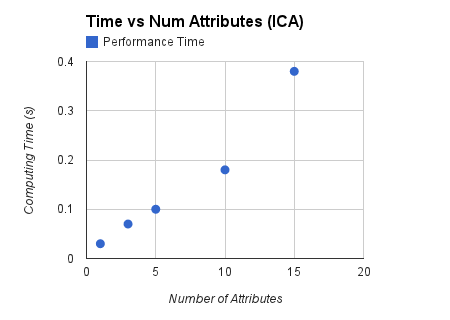
\includegraphics[width=3.5in]{charts/time_vs_attr_ica.png}
  \caption{Effect of number of attributes on computing time}
  \label{fig:timevsattr}
\end{figure}
\begin{figure}[ht]
  \centering
  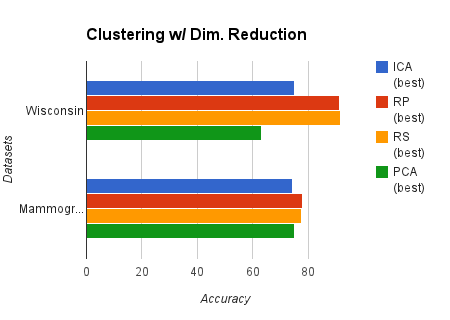
\includegraphics[width=3.5in]{charts/clust_dim_red_2.png}
  \caption{Clustering after Dimensionality Reduction Results for Expectation Maximization (EM)}
  \label{fig:clustdimred2}
\end{figure}

For the results in this section, I hypothesized the results for the Mammography dataset would perform well due to their lower number of attributes. The results demonstrated this thought but in a way which I did not expect. The results demonstrated a very high level of precision for the Mammography dataset whilst the Wisconsin dataset produced the exact opposite. Reasonably enough the random algorithms were precise (because we were picking the best random result), but ICA and PCA performed poorly in comparison. This further demonstrates the difficulty of dimensionality reduction without a loss of performance. Yet again, the computing time was much better after the reduction of dimensions, but the performance in this case was very poor. The results can be seen in Figure~\ref{fig:clustdimred2}.

\section{Neural Network Learner}
In order to evaluate all of the clustering and dimensionality reduction algorithms, I ran a neural network learner on all of the results. The first interesting phenomenon that the neural network test demonstrates is the computing time vs accuracy tradeoff. As can be demonstrated in Figure~\ref{fig:perftime}, having more components will generally lead to better accuracy and classification, but this reaches a ceiling at n attributes. It is important to note here that having bad attributes does not have a huge effect because this is a neural network which weighs the parameters adequately to obtain the optimal performance, which is why we see such an increase in performance. In this sense, more information is put simply, better.
\begin{figure}[ht]
  \centering
  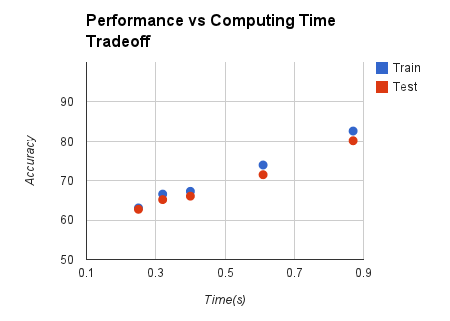
\includegraphics[width=3.5in]{charts/accuracy_time_tradeoff.png}
  \caption{The increase in computing time is caused by the increased number of parameters in ICA. This figure augments Figure ~\ref{fig:timevsattr} which demonstrates the number of attributes affects the computing time. Although the time is increased, it comes with the benefit of accuracy, which is a classic tradeoff in computing problems.}
  \label{fig:perftime}
\end{figure}
\subsection{Dimensionality Reduction}

\begin{table}
    \begin{tabular}{|c|c|c|}
  \hline
        Dim. Red Algorithm    & Accuracy (train)   & Accuracy (test)   \\ \hline
        ICA                   & 82.60\%            & 80.14\%           \\ 
        PCA                   & 98.41\%            & 97.19\%           \\ 
        RP                    & 97.01\%            & 96.66\%           \\ 
        RS                    & 98.24\%            & 97.71\%           \\
        None                  & 98.94\%            & 97.89\%           \\

  \hline \end{tabular}
  \caption {Comparison of Algorithm Performance - None is the ground truth. In this case, the original dataset performes better, but its important to highlight that PCA and RS run at significantly faster rates for a small tradeoff in accuracy.} \label{tb:perfdesc}
  \label{tb:perf}
\end{table}
Out of all of the possible dimensionality reduction parameters, we chose the best to be represented in Table~\ref{tb:perf}. These small tradeoffs in accuracy can be accounted for by illustrating the amount that the algorithms take to train. Specifically, the original algorithm ran at 2.41s, and RS and PCA run at 0.96 and 0.67s respectively. You can imagine this becoming incredibly important for massive datasets, which encompasses the purpose of dimensionality reduction. 
\subsection{Clustering with Dimensionality Reduction}
I was unable to conduct the experiments for adding clustering to the dimensionality reduction algorithms due to time constraints. However, I felt that analyzing the potential effects of it would be intriguing. 

Primarily, I think neural networks would be heavily affected by it due to the inherent separation that those attributes would cause. However, this is a double edged sword due to the fact that the accuracy of none of the clusters is better than the accuracy of the original data. Although the overlap of the clusters with the original attributes could produce better accuracy, it is most likely to be hurt by the clusters because the clusters fail at properly mapping to the binary classification. However, the more intriguing approach would be to use the expectation maximization cluster, where the algorithm generates a number of clusters based on the data. This experiment may provide better results because the accuracy within the clusters that actually categorize the data would be weighed heavily, whilst the clusters that do not identify the data appropriately would simply be less relevant to the neural network. It would therefore be smart to add \emph{n} binary attributes for the \emph{n} clusters that the EM algorithm creates in order to benefit the neural network the most.
\section{Conclusion}
In conclusion, dimensionality reduction and clustering algorithm serve the main purpose of decreasing the processing time of algorithms. In the specific case of our datasets, it does not seem to be the case that accuracy was improved, but there were cases in which performance remained virtually the same, whilst running significantly faster. In terms of the datasets, it seems to be the case that the Wisconsin dataset has much better classification attributes. However, this may be due to the sheer number of attributes that it has, or to the fact that the Mammography dataset is missing data. It is difficult to conclude which of these is at fault or to blame, but further experiments would be needed to reach a stronger hypothesis in this scenario.
\section{Future Work}
For future work, I would like to experiment heavily with finding the ideal space between performance time and accuracy. I think dimensionality reduction and clustering provide a fascinating medium that allow you to simplify problems with small sacrifices to your accuracy. Some algorithms perform better than others in terms of precision for this scenario, but it is important to highlight that altering the appropriate parameters is still incredibly relevant in these algorithms.

Further, although this data is currently not available, it would be interesting to somehow be able to combine the two breast mass datasets in order to analyze the best parameters for categorization. An ideal start to this problem would be to attempt the classification problem using only one attribute, and to then perform this for each attribute (to see the effect that each independent attribute has on classification). That way, I may be able to advise medical professionals which parameters would allow for the best classification.
\section*{Acknowledgements}
First, I'd like to recognize the work by ~\cite{Frank+Asuncion:2010} for the UCI Machine Learning Dataset Repository which contained both of the datasets discussed in this paper. First i'd like to recognize the University of Wisconsin for their efforts in the Wisconsin Breast Cancer Diagnostic dataset. Secondly, I'd like to recognize the dataset introduced by ~\cite{elter2007prediction} which takes a unique approach at breast mass diagnosis. Lastly, it is incredibly important to acknowledge the ABAGAIL Java programming library which provided our implementation of the ICA dimensionality reduction algorithm, and the use of Weka~\cite{Hall_weka:2010} for every other algorithm present in this paper.
\bibliographystyle{acmsiggraph}
\bibliography{machine_learning_p3}
\end{document}
